\subsection{XT30 Female Connector}

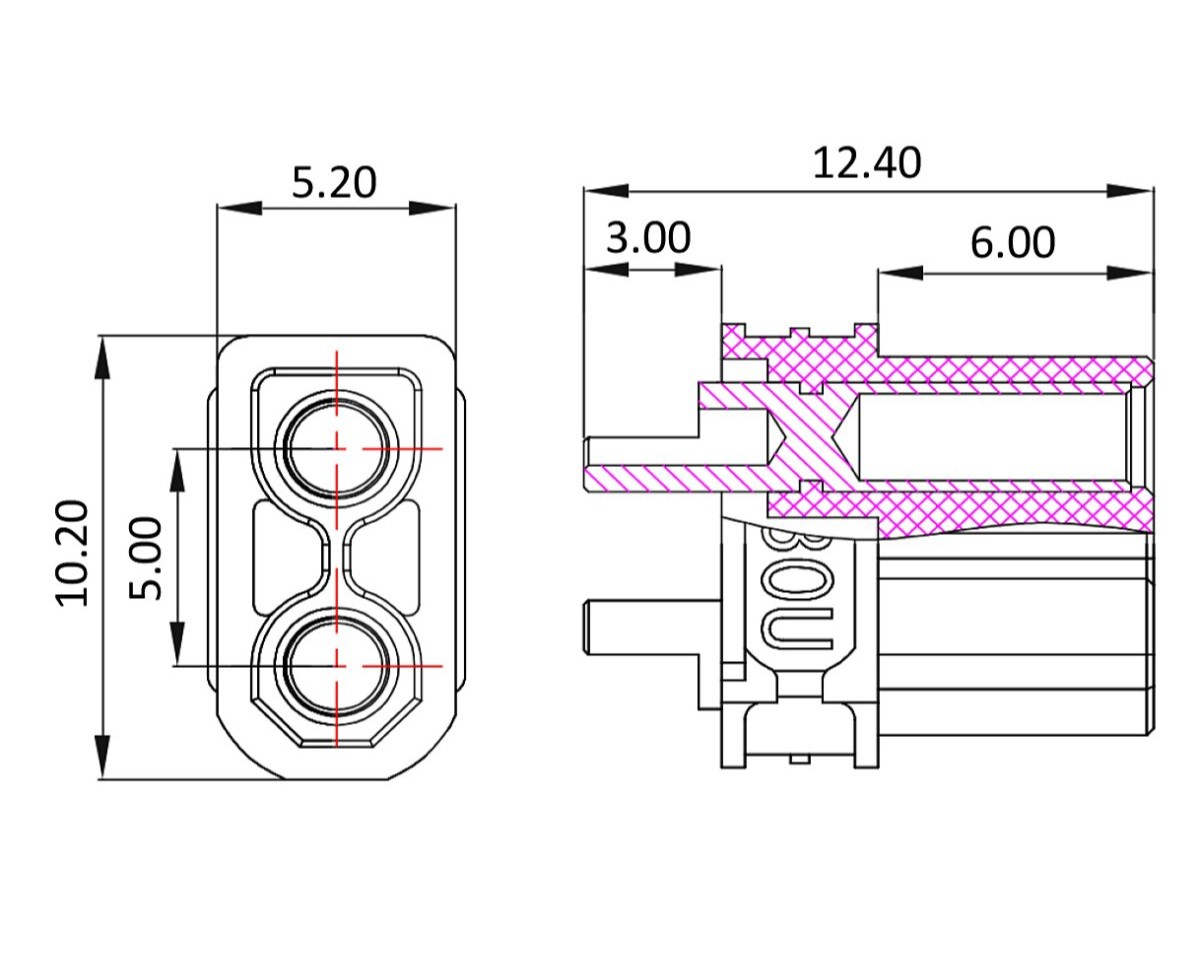
\includegraphics[width=\textwidth]{contents/figures/xt30_f.jpg}

The datasheet of the XT-series of connectors can be found \href{https://www.lcsc.com/datasheet/lcsc_datasheet_2304140030_Changzhou-Amass-Elec-XT30U-F_C99102.pdf}{\textbf{\underline{here}}}.
The table below is only an extract of the most important information, to be used as standalone reference and also in case the URL above fails.

\begin{table}[h] %Float specifier check: passed!
    \begin{tabular}{rlrl}
         Item No.:&  XT30U-F &  Contact Resistance:& $0.70m \Omega$\\
         Color:&  Black \& Yellow&  Max. Voltage:& $500V$\\
         Contact Material:&  Gold plated brass&  Continous Current:& $15A$\\
         Isolation Material:&  PA (Nylon)&  Max. Current:& $30A$\\
         Flammability:&  94V-0&  Mating Cycles:& 1000\\
         Certifications:&  CE/UL&  Temperature Range:& -20°C - 120°C\\
    \end{tabular}
    \caption{XT30 female connector and its electrical and mechnanical parameters.}
    \label{tab:xt30_f_specs}
\end{table}

\clearpage %PAGE SPECIFIER
    
\subsection{XT30 Male Connector}

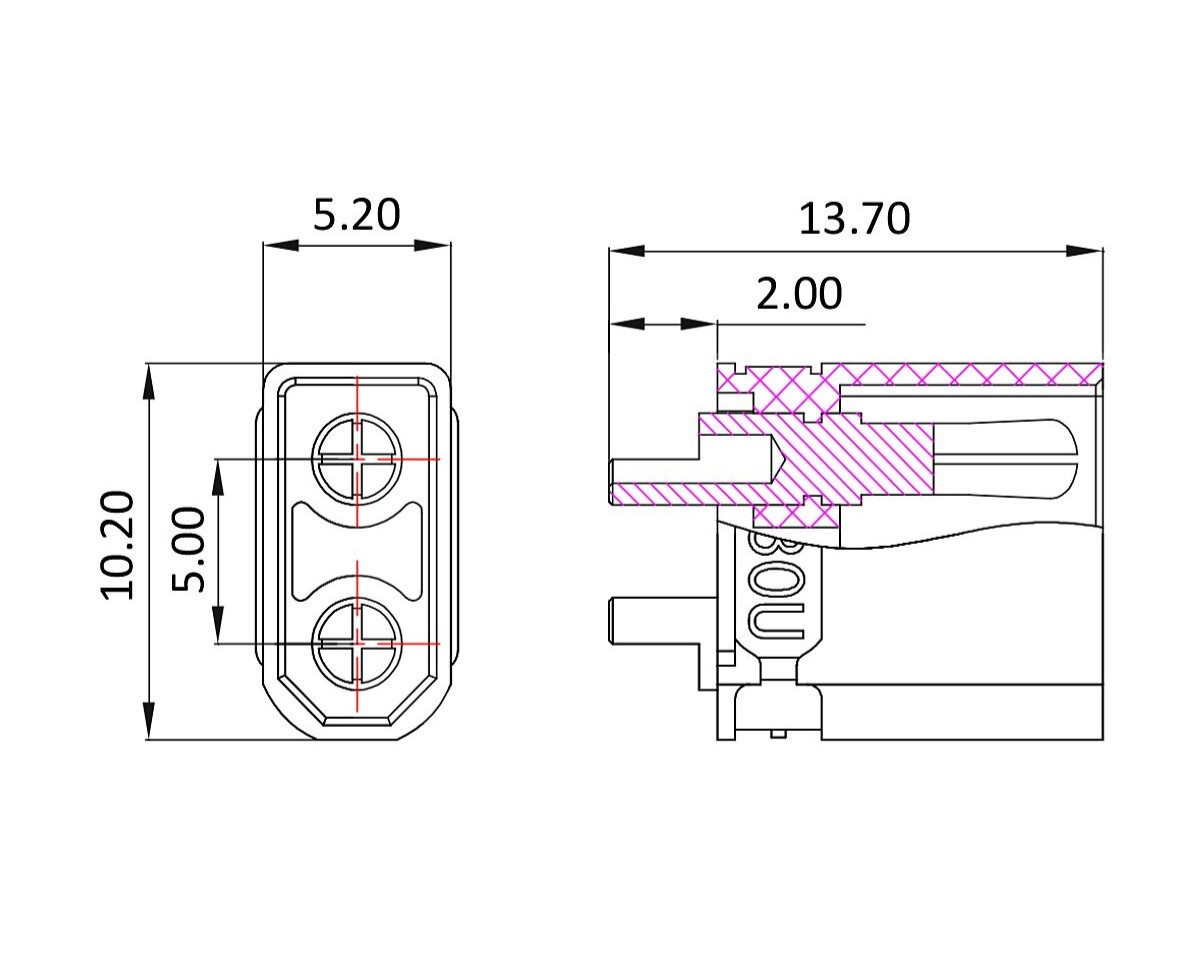
\includegraphics[width=\textwidth]{contents/figures/xt30_m.jpg}

The datasheet of the XT-series of connectors can be found \href{https://www.lcsc.com/datasheet/lcsc_datasheet_2304140030_Changzhou-Amass-Elec-XT30U-F_C99101.pdf}{\textbf{\underline{here}}}.
The table below is only an extract of the most important information, to be used as standalone reference and also in case the URL above fails.

\begin{table}[h] %Float specifier check: passed!
    \begin{tabular}{rlrl}
         Item No.:&  XT30U-M &  Contact Resistance:& $0.70m \Omega$\\
         Color:&  Black \& Yellow&  Max. Voltage:& $500V$\\
         Contact Material:&  Gold plated brass&  Continous Current:& $15A$\\
         Isolation Material:&  PA (Nylon)&  Max. Current:& $30A$\\
         Flammability:&  94V-0&  Mating Cycle& 1000\\
         Certification&  CE/UL&  Temperature Range:& -20°C - 120°C\\
    \end{tabular}
    \caption{XT30 male connector and its electrical and mechnanical parameters.}
    \label{tab:xt30_m_specs}
\end{table}

\clearpage %PAGE SPECIFIER

\subsection{XT60 Female Connector}

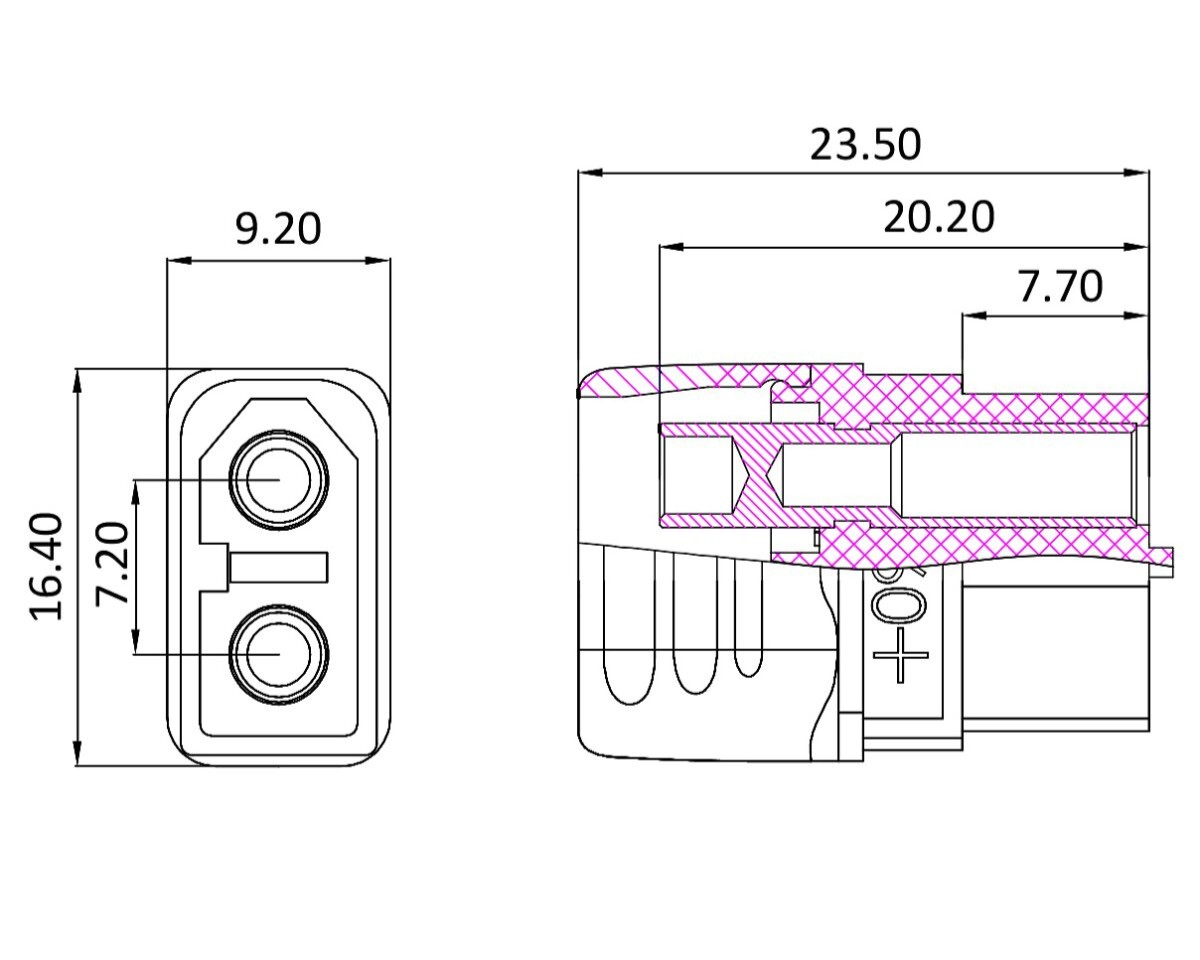
\includegraphics[width=\textwidth]{contents/figures/xt60_f.jpg}

The datasheet of the XT-series of connectors can be found \href{https://www.lcsc.com/datasheet/lcsc_datasheet_1810251322_Changzhou-Amass-Elec-XT60-F_C98734.pdf}{\textbf{\underline{here}}}.
The table below is only an extract of the most important information, to be used as standalone reference and also in case the URL above fails.

\begin{table}[h] %Float specifier check: passed!
    \begin{tabular}{rlrl}
         Item No.:&  XT60U-F &  Contact Resistance:& $0.55m \Omega$\\
         Color:&  Black \& Yellow&  Max. Voltage:& $500V$\\
         Contact Material:&  Gold plated brass&  Continous Current:& $30A$\\
         Isolation Material:&  PA (Nylon)&  Max. Current:& $60A$\\
         Flammability:&  94V-0&  Mating Cycles:& 1000\\
         Certifications:&  CE/UL&  Temperature Range:& -20°C - 120°C\\
    \end{tabular}
    \caption{XT60 Female Connector and its electrical and mechnanical parameters.}
    \label{tab:xt60_f_specs}
\end{table}

\clearpage %PAGE SPECIFIER

\subsection{XT60 Male Connector}

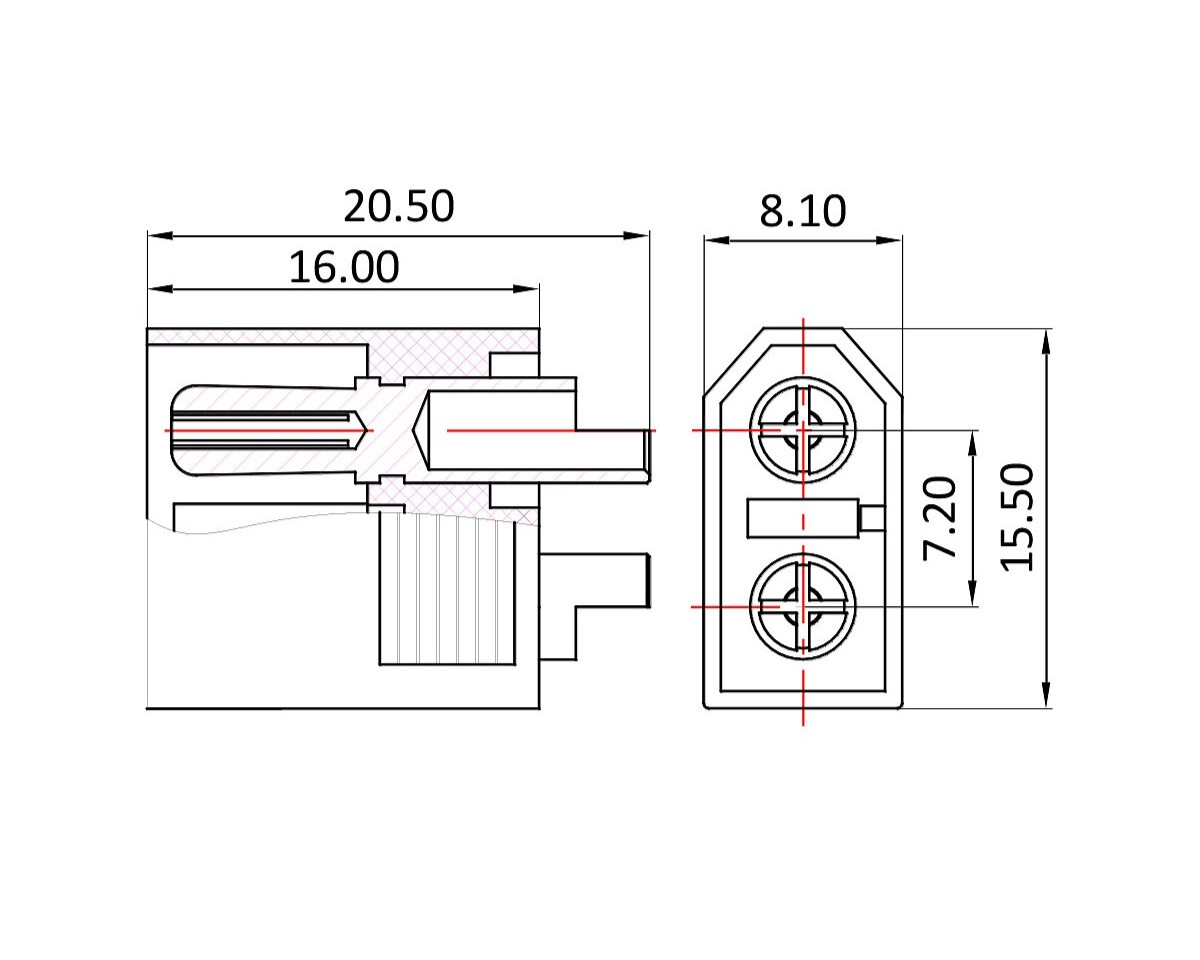
\includegraphics[width=\textwidth]{contents/figures/xt60_m.jpg}

The datasheet of the XT-series of connectors can be found \href{https://www.lcsc.com/datasheet/lcsc_datasheet_1810251322_Changzhou-Amass-Elec-XT60_C98733.pdf}{\textbf{\underline{here}}}.
The table below is only an extract of the most important information, to be used as standalone reference and also in case the URL above fails.

\begin{table}[h] %Float specifier check: passed!
    \begin{tabular}{rlrl}
         Item No.:&  XT60U-M &  Contact Resistance:& $0.55m \Omega$\\
         Color:&  Black \& Yellow&  Max. Voltage:& $500V$\\
         Contact Material:&  Gold plated brass&  Continous Current:& $30A$\\
         Isolation Material:&  PA (Nylon)&  Max. Current:& $60A$\\
         Flammability:&  94V-0&  Mating Cycles:& 1000\\
         Certifications:&  CE/UL&  Temperature Range:& -20°C - 120°C\\
    \end{tabular}
    \caption{XT60 Female Connector and its electrical and mechnanical parameters.}
    \label{tab:xt60_f_specs}
\end{table}

\clearpage %PAGE SPECIFIER

\subsection{XT90 Female Connector}

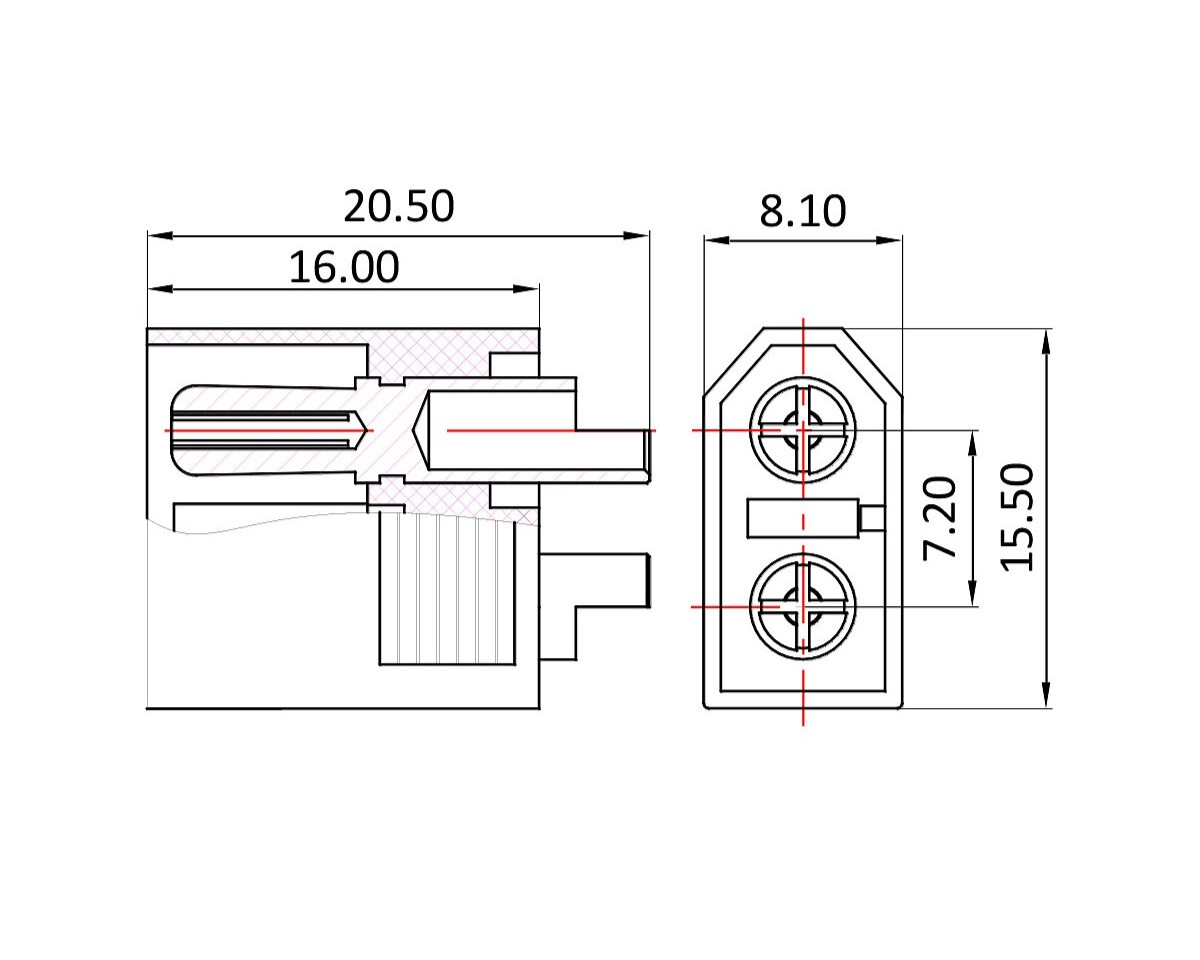
\includegraphics[width=\textwidth]{contents/figures/xt60_m.jpg}

The datasheet of the XT-series of connectors can be found \href{https://www.lcsc.com/datasheet/lcsc_datasheet_1810251322_Changzhou-Amass-Elec-XT60_C98733.pdf}{\textbf{\underline{here}}}.
The table below is only an extract of the most important information, to be used as standalone reference and also in case the URL above fails.

\begin{table}[h] %Float specifier check: passed!
    \begin{tabular}{rlrl}
         Item No.:&  XT60U-M &  Contact Resistance:& $0.55m \Omega$\\
         Color:&  Black \& Yellow&  Max. Voltage:& $500V$\\
         Contact Material:&  Gold plated brass&  Continous Current:& $30A$\\
         Isolation Material:&  PA (Nylon)&  Max. Current:& $60A$\\
         Flammability:&  94V-0&  Mating Cycles:& 1000\\
         Certifications:&  CE/UL&  Temperature Range:& -20°C - 120°C\\
    \end{tabular}
    \caption{XT60 Female Connector and its electrical and mechnanical parameters.}
    \label{tab:xt60_f_specs}
\end{table}

\clearpage %PAGE SPECIFIER
